\documentclass[11pt]{article}
\usepackage[UTF8]{ctex}
\usepackage[a4paper]{geometry}
\geometry{left=2.0cm,right=2.0cm,top=2.5cm,bottom=2.5cm}

\usepackage{comment}
\usepackage{booktabs}
\usepackage{graphicx}
\usepackage{diagbox}
\usepackage{amsmath,amsfonts,graphicx,amssymb,bm,amsthm}
%\usepackage{algorithm,algorithmicx}
\usepackage[ruled]{algorithm2e}
\usepackage[noend]{algpseudocode}
\usepackage{fancyhdr}
\usepackage{tikz}
\usepackage{graphicx}
\usetikzlibrary{arrows,automata}
\usepackage{hyperref}
\usepackage{float}
\usepackage{tikz}
\usepackage{tikz-qtree}

\setlength{\headheight}{14pt}
\setlength{\parindent}{0 in}
\setlength{\parskip}{0.5 em}

\newtheorem{theorem}{Theorem}
\newtheorem{lemma}[theorem]{Lemma}
\newtheorem{proposition}[theorem]{Proposition}
\newtheorem{claim}[theorem]{Claim}
\newtheorem{corollary}[theorem]{Corollary}
\newtheorem{definition}[theorem]{Definition}
\newtheorem*{definition*}{Definition}

\newenvironment{problem}[2][Problem]{\begin{trivlist}
		\item[\hskip \labelsep {\bfseries #1}\hskip \labelsep {\bfseries #2.}]}{\hfill$\blacktriangleleft$\end{trivlist}}
\newenvironment{answer}[1][Answer]{\begin{trivlist}
		\item[\hskip \labelsep {\bfseries #1.}\hskip \labelsep]}{\hfill$\lhd$\end{trivlist}}

\begin{document}
	
	\pagestyle{fancy}
	\lhead{Peking University}
	\chead{}
	\rhead{Introduction to the Theory of Computation, 2024 Spring}
	
	\begin{center}
		{\LARGE \bf Homework 1}\\
		{Due: 2024-3-22 23:59 \quad$|$\quad 6 Problems, 100 Pts}
		{Name: 胡宇阳, ID: 2200013065}
	\end{center}
	\begin{problem}{1.(10 points)}
		$~$
		
		(1) (5 points) Give a DFA recognizing the following language. The alphabet is $\{0, 1\}$.
		\begin{align*}
			\{w \mid w \mbox{ contains exactly two }0\mbox{s and at least one }1\}
		\end{align*}
		(2) (5 points) Give an NFA recognizing the language $0^*1^*0^+$ with four states (including a reject state). The alphabet is $\{0, 1\}$.
	\end{problem}
	\begin{answer}
		(1)	
		
		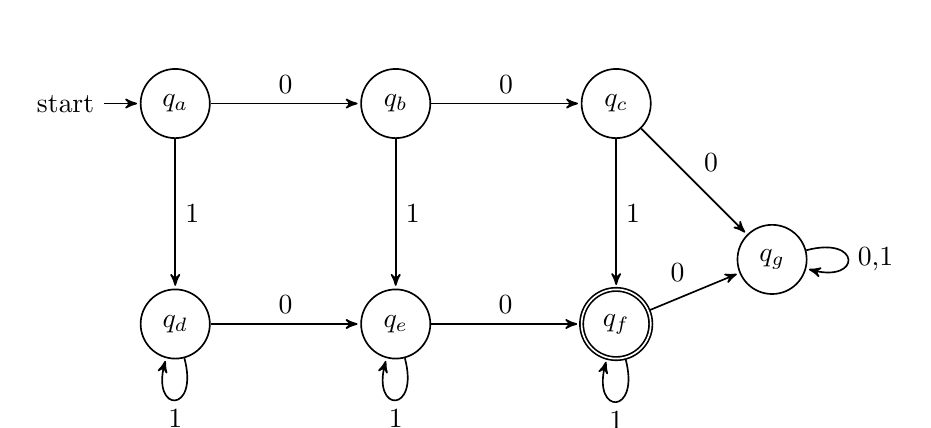
\begin{tikzpicture}[->,>=stealth',shorten >=1pt,auto,node distance=2.8cm,semithick]
		\tikzstyle{every state}=[fill=white ,draw=black,text=black]
		\node[initial,state] (A) {$q_a$};
		\node[state] (B) [right of=A] {$q_b$};
		\node[state] (C) [right of=B] {$q_c$};
		\node[state] (D) [below of=A] {$q_d$};
		\node[state] (E) [below of=B] {$q_e$};
		\node[accepting,state] (F) [below of=C] {$q_f$};
		\node[state] (G) [below right of=C] {$q_g$};
		\path 
		(A) edge node {0} (B)
			edge node {1} (D)
		(B) edge node {0} (C)
			edge node {1} (E)
		(C) edge node {0} (G)
			edge node {1} (F)
		(D) edge node {0} (E)
			edge [loop below] node {1} (D)
		(E) edge node {0} (F)
			edge [loop below] node {1} (E)
		(F) edge node {0} (G)
			edge [loop below] node {1} (F)
		(G) edge [loop right] node {0,1} (G);
		\end{tikzpicture}
		
		(2)
		
		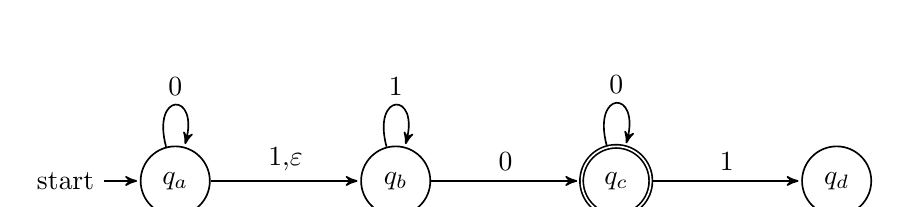
\begin{tikzpicture}[->,>=stealth',shorten >=1pt,auto,node distance=2.8cm,semithick]
		\tikzstyle{every state}=[fill=white ,draw=black,text=black]
		\node[initial,state] (A) {$q_a$};
		\node[state] (B) [right of=A] {$q_b$};
		\node[accepting,state] (C) [right of=B] {$q_c$};
		\node[state] (D) [right of=C] {$q_d$};
		\path 
		(A) edge [loop above] node {0} (A)
			edge node {1,$\varepsilon$} (B)
		(B) edge [loop above] node {1} (B)
			edge node {0} (C)
		(C) edge [loop above] node {0} (B)
			edge node {1} (D);
		\end{tikzpicture}
	\end{answer}
	\begin{problem}{2.(20 points)}
		For any string $w = w_1w_2\cdots w_n$, the reverse of $w$, written $w^R$, is the string $w$ in reverse
		order, $w_n\cdots w_2w_1$. For any language $A$, let $A^R = \{w^R\mid w\in A\}$. Show that if $A$ is regular, so is $A^R$.
	\end{problem}
	\begin{answer}
		\textcircled{1} 由于 $A$ 为正则语言, 存在 DFA  $M=(Q,\Sigma,\delta,q_0,F)$, $M$ 识别 $A$.
		
		则构造 NFA $\bar{M}=(\bar{Q},\bar{\Sigma},\bar{\delta},\bar{q}_0,\bar{F})$, 满足 $\bar{Q}=Q\cup S_0$, $\bar{\Sigma}=\Sigma\cup\{\varepsilon\},\bar{q}_0=S_0,\bar{F}=q_0$.
		
		$\bar{\delta}$ 是满足 $\forall q_1\in Q\wedge w\in\Sigma, q_2=\delta(q_1,w)\Leftrightarrow q_1\in\bar{\delta}(q_2,w)$ 和 $\forall q\in F,q\in \bar{\delta}(S_0,\varepsilon)$ 的最小集合.
		
		\textcircled{2} 下证 $\bar{M}$ 接受 $A^R$ 中的字符串:
		
		$\forall w=w_1w_2\cdots w_n,w_i\in\Sigma$, 若 $w$ 可被 $A$ 识别, 则 $\exists r_0,r_1,\cdots,r_n\in Q$, $(r_0=q_0)\wedge (r_{i+1}=\delta(r_i,w_{i+1}),i=0,1,\cdots,n-1)\wedge (r_n\in F)$.
		
		$r_n\in F,\bar{q}_0=S_0~\Rightarrow~ r_n\in\bar{\delta}(\bar{q}_0,\varepsilon)$
		
		$r_{i+1}=\delta(r_i,w_{i+1}),i=0,1,\cdots,n-1~\Rightarrow~r_i\in\bar{\delta}(r_{i+1},w_{i+1}),i=0,1,\cdots,n-1$
		
		$\bar{F}=q_0,r_0=q_0\Rightarrow r_0\in\bar{F}$
		
		由 accept 的定义, $\bar{M}$ 识别 $A^R$.
		
		\textcircled{3} 下证 $\bar{M}$ 拒绝 $A^R$ 外的字符串，即证 $w$ 被 $A^R$ 接受可以推出 $w^R$ 在 $A$ 中.
		
		$\forall w=w_1w_2\cdots w_n,w_i\in\{\Sigma\cup\varepsilon\}$, 若 $w$ 可被 $A^R$ 识别, 则 $\exists r_0,r_1,\cdots,r_n\in Q$, $(r_0=q_0)\wedge (r_{i+1}\in\delta(r_i,w_{i+1}),i=0,1,\cdots,n-1)\wedge (r_n\in F)$.
		
		由于 $\bar{M}$ 只有与 $S_0$ 相连的边才识别 $\varepsilon$, 所以只有 $w_1=\varepsilon$, $w_2,\cdots,w_n\neq\varepsilon$ 才成立. 所以 $w_2w_3\cdots w_n$可以被 $\bar{M}$ 接受.
		
		$r_n=\bar{F},\bar{F}=q_0~\Rightarrow~r_n=q_0$
		
		$r_{i+1}\in\bar{\delta}(r_i,w_{i+1}),i=0,1,\cdots,n-1~\Rightarrow~r_i=\delta(r_{i+1},w_{i+1}),i=1,\cdots,n-1$
		
		$\forall q\in F,q\in \bar{\delta}(S_0,\varepsilon)\wedge r_1=\bar\delta(S_0,\varepsilon)\Rightarrow r_1\in F$
		
		由 accept 的定义, $M$ 接受 $w_nw_{n-1}\cdots w_2$, 证毕.
	\end{answer}
	\begin{problem}{3.(20 points)}
		Let $A$ be any language. Define DROP-OUT($A$) to be the language containing all strings
		that can be obtained by removing one symbol from a string in $A$. Thus, DROP-OUT($A$) = $\{a\mid\exists y \in \Sigma, \exists x, z\in\Sigma^*: xyz\in A\bigwedge a = xz\}$. Show that the class of regular languages is closed under the
		DROP-OUT operation. In other words, if $A$ is a regular language, so is DROP-OUT($A$).
	\end{problem}
	\begin{answer}
		\textcircled{1} 由于 $A$ 为正则语言, 存在 DFA  $M=(Q,\Sigma,\delta,q_0,F)$, $M$ 识别 $A$.
		
		则构造 NFA $\bar{M}=(\bar{Q},\bar{\Sigma},\bar{\delta},\bar{q}_0,\bar{F})$, 满足 $\bar{Q}=Q\times\{a,b\}$, $\bar{\Sigma}=\Sigma,\bar{q}_0=(q_0,a),\forall q\in F,(q,b)\in\bar{F}$.
		
		$\bar{\delta}$ 是满足 $\forall q_1\in Q\wedge w\in\Sigma, q_2=\delta(q_1,w)\Leftrightarrow (q_2,a)\in\bar{\delta}((q_1,a),w),(q_2,b)\in\bar{\delta}((q_1,b),w),(q_2,b)\in\bar{\delta}((q_1,a),\varepsilon)$ 的最小集合.
		
		\textcircled{2} 下证 $\bar{M}$ 接受 DROPOUT($A$):
		
		设字符串 $A=w_1w_2\cdots w_n$ 能被 $M$ 识别, 则 $q_{i+1}=\delta(q_i,w_{i+1})$.
		
		对于 DROPOUT($A$) 中任意一个字符串 $w_1w_2\cdots w_{t-1}w_{t+1}\cdots w_n$, 
		
		$(q_i,a)=\bar\delta((q_{i-1},a),w_i),i=1,2,\cdots,t-1$,
		
		$(q_t,b)=\bar\delta((q_{t-1},a),\varepsilon))$
		
		$(q_i,b)=\bar\delta((q_{i-1},b),w_i),i=t+1,t+2,\cdots,n$,
		
		所以 $\bar{M}$ 接受 $w_1w_2\cdots w_{t-1}w_{t+1}\cdots w_n$
	
		\textcircled{3} 下证被 $\bar{M}$ accept 的字符串在 DROPOUT($A$) 中:
		
		对于被 DROPOUT($A$) accept 的字符串 $w_1w_2\cdots w_n$, $\exists \mbox{对其补充} \varepsilon \mbox{的方法变为}  x_1x_2\cdots x_m, r_0,r_1,\cdots,r_m\in\bar{Q}, r_i=\bar\delta(r_{i-1},x_i),i=1,2,\cdots,m$.
		
		由于从 $(\sim,a)$ 出发, 在 $(\sim,b)$ 结束, 且只有一次从 $(\sim,a)$ 到 $(\sim,b)$ 的机会, 所以 $m=n+1$ 且 $\exists t,x_1x_2\cdots x_m=w_1w_2\cdots w_t\varepsilon w_{t+1}\cdots w_n$.
		
		则 $1\sim t-1$ 时 $r_i=\bar\delta(r_{i-1},w_i)$, $r_i\in(\sim,a)$
		
		$t+1\sim m$ 时 $r_i=\bar\delta(r_{i-1},w_i)$, $r_i\in(\sim,b)$.
		
		将 NFA 对应回原来的 DFA, $1\sim t-1$ 时 $q_i=\delta(q_{i-1},w_i)$, 
		
		$t+1\sim m$ 时 $q_i=\delta(q_{i-1},w_i)$
		
		设 $q_{t}=\delta(q_{t-1},z)$, 则 $M$ 接受 $w_1w_2\cdots w_tzw_{t+1}\cdots w_n$. 
		
		由于 $w_1w_2\cdots w_n$ 在 DROPOUT($A$) 中, $w_1w_2\cdots w_tzw_{t+1}\cdots w_n$ 在 $A$ 中.
	\end{answer}
	\begin{problem}{4.(20 points)}
		For a language $A$, define an equivalence relation between two strings: $x \equiv y$ means
		$\forall z\in\Sigma^* : xz\in A\Leftrightarrow yz\in A$. This allows the set $\Sigma^*$
		to be divided into different equivalence
		classes.
		
		For example, if $A = \{w \mid w \mbox{contains exactly two }0\mbox{s and at least one }1\}$, then $1\equiv1111, 101\equiv110$, but $1\not\equiv011$.
		
		(1) (5 points) How many different equivalence classes are there for $A$ in the above example?
		
		(2) (5 points) Prove that for every regular language $A$, $\Sigma^*$ can be divided into a finite number of equivalence classes.
		
		(3) (5 points) Prove that if $\Sigma^*$ can be divided into a finite number of equivalence classes for a language $A$, then $A$ is a regular language.
		
		(4) (5 points) With the above conclusions, prove $A$ = $\{0^n1^n\mid n\in\mathbb{N}\}$ is not a regular language.
	\end{problem}
	\begin{answer}
		(1) 7个, 没有1和0, 有1没有0, 没有1有一个0, 有1有一个0, 没有1有两个0, 有1有两个0, 有3个0.
		
		(2) 由于 $A$ 为正则语言, 则存在一个 state 数量最少的 DFA $M=(Q,\Sigma,\delta,q_0,F)$, $M$ 识别 $A$.
		
		下证任意字符串 $s,\bar{s}$, 
		
		由定义, $\exists r_0,r_1,\cdots,r_n,\bar{r}_0,\bar{r}_1,\cdots,\bar{r}_m \in Q$, $r_0=\bar{r}_0=q_0,\delta(r_i,w_{i+1})=r_{i+1},\delta(\bar{r}_i,w_{i+1})=\bar{r}_{i+1}$
		
		$s$ 和 $\bar{s}$ 在同一个等价类 $\Leftrightarrow$ $r_n=\bar{r}_m$
		
		对于 $q\in Q,z=w_1w_2\cdots w_n$, 定义 $\delta^n(q,z)=\delta(\delta(\cdots\delta(q,w_1)\cdots w_{n-1})w_n)$.
		
		\textcircled{1} “$\Leftarrow$” 
		
		若 $r_n=\bar{r}_m$,
		 
		$\therefore\forall z=w_0,w_1,\cdots,w_t$, $\delta^t(r_n,z)=\delta^t(\bar{r}_m,z)$
		
		$\therefore \delta^{n+r}(q_0,sz)=\delta^{m+r}(q_0,\bar{s}z)$
		
		$\therefore s,\bar{s}$ 在同一个等价类.
		
		\textcircled{2} “$\Rightarrow$” 
		
		若 $r_n\neq\bar{r}_m$, 而	$s$ 和 $\bar{s}$ 在同一个等价类, 则 $\forall x\in\Sigma,\delta(r_n,x)=\delta(\bar{r}_m,x)$, 可以将 $r_n$ 和 $\bar{r}_m$ 合并为同一个 state, 而不会改变其识别的语言, 与 state 数量最少矛盾.
		
		(3) \textcircled{1} 设 $\Sigma^*$ 一共 $n$ 个等价类 (用代表元表示) $[x_1],[x_2],\cdots,[x_n]$, 则构造一个 NFA $M=(Q,\Sigma,\delta,q_0,F)$ 满足如下条件:
		
		$Q=\{Q_1,Q_2,\cdots,Q_n\}$.
		
		$\Sigma$ 不变.
		
		$q_0=\{Q_i\mid \varepsilon\in x_i\}$
		
		$F=\{Q_i\mid\exists x\in Q_i,x\in A\}$, 由于等价类的性质, 取 $z=0$ 时可得到一个状态对应的等价类只有都不接受和都接受两种状态.
		
		$\delta$ 满足 $\forall q_i\in Q,x\in[x_i],w\in\Sigma, [x_iw]\in\delta(q_i,w)$ (通过字符串的拼接进行连接).
		
		\textcircled{2} 下证 $M$ 识别 $A$: 对于 $s=w_1w_2\cdots w_n\in\Sigma^*$, 存在 $r_0,r_1,\cdots,r_n\in Q$, $r_i=[w_1w_2\cdots w_i]$, 使得 $r_i=\delta(r_{i-1},w_i)$.
		
		由 $F$ 的定义, 所以 $M$ 识别 $A$.
		
		(4) 对于字符串 $s_1=0^n1^m,m\leq n$, $\forall s_2\in\Sigma^*,s_1s_2\in A~\Leftrightarrow~s_2=1^{n-m}$.
		
		$\therefore s_1=0^n1^m,n-m=C\geq 0$ 在同一个等价类, 且与 $n-m$ 不同的 $0^n1^m$ 字符串不在同一个等价类.
		
		$\therefore 0^11^1,0^21^1,0^31^1,\cdots$ 均在不同的等价类.
		
		由 (2) , $A$ 不是正则语言.
	\end{answer}
	\begin{problem}{5.(10 points)}
		Prove that the following languages are not regular.
		
		(1) (5 points) $\{0^m1^n\mid m \mbox{ and } n \mbox{ are coprime}\}$.
		
		(2) (5 points) $\{w\mid w\in \{0, 1\}^*\mbox{ is not a palindrome}\}$. Here a palindrome is a string that reads the same forward and backward.
	\end{problem}
	\begin{answer}
		(1) 由第四题结论, 将 $A=\{0^m1^n\mid m \mbox{ and } n \mbox{ are coprime}\}$ 分为不同的等价类. 对于 $0^m1^n$, 若 $m$ 为质数, 则 $1$ 的个数必须为 $m$ 的倍数才满足条件, 
		
		也就是说对于 $s_1=0^m1^n_1,s_2=0^m1^n_2$, $s_1$ 和 $s_2$ 在同一个等价类 $\Leftrightarrow$ $n_1\equiv n_2(mod m)$.
		
		所以 $0^m1^n$ 有 $m$ 个同余类, 而质数是无限的, 所以有无限个同余类, $A$ 不是正则语言.
		
		(2) 由第四题结论, 将 $A=\{w\mid w\in \{0, 1\}^*\mbox{ is not a palindrome}\}$ 分为不同的等价类. 对于字符串 $s=0^n1$, $z=10^m$, $sz$ 为回文串 $\Leftrightarrow$ $m=n$

        所以 $01,001,0001\cdots$ 均在不同的等价类, 所以有无限个同余类, $A$ 不是正则语言.
	\end{answer}
	\begin{problem}{6.(20 points)}
		Let the rotational closure of language $A$ be $RC(A) = \{yx\mid xy \in A\}$.
		
		(1) (10 points) Show that for any language $A$, we have $RC(A) = RC(RC(A))$.
		
		(2) (10 points) Show that the class of regular languages is closed under rotational closure. In other words, if $A$ is a regular language, so is $RC(A)$.
	\end{problem}
	\begin{answer}
		(1) 因为 $x,y$ 可以取空集, 所以显然 $RC(A) \subseteq RC(RC(A))$. 下证 $RC(RC(A)) \subseteq RC(A)$.

        对于 $str\in RC(RC(A)), \exists x,y,z, xyz\in A \wedge(yzx\in RC(RC(A)) \vee zxy\in RC(RC(A)))$

        而 $x(yz)\in A \Rightarrow (yz)x\in RC(A)$, $(xy)z\in A \Rightarrow z(xy)\in RC(A)$, $\therefore RC(RC(A)) \subseteq RC(A)$.

        $\therefore RC(A) = RC(RC(A))$.
        
        (2) 若 $A$ 为正则语言, 则存在 DFA $M=(Q,\Sigma,\delta,q_0,F)$, $M$ 识别 $A$.
        
        $\forall q\in Q$, 将 $M$ 拆成两个 DFA $M_{q1}=(Q,\Sigma,\delta,q_0,q),M_{q2}=(Q,\Sigma,\delta,q,F)$, 将 $M_{q2}$ 的接受状态 和 $M_{q1}$ 的起始状态用 $\varepsilon$ 组合起来, 得到 NFA $M_q$, 其识别语言 $A_q$.
        
        下证 $\bigcup_{q\in Q} A_q=RC(A)$
        
        \textcircled{1} 对于 $x=w_1w_2\cdots w_k,y=w_{k+1}w_{k+2}\cdots w_n,xy\in A$, 则 $\exists r_0,r_1,\cdots,r_n\in Q,r_i=\delta(r_{i-1},w_i)$.
        
        设 $q=r_k$, 由 accept 的定义知 $M_{q1}$ 接受 $x$, $M_{q2}$ 接受 $y$, 则 $M_q$ 接受 $yx\in RC(A)$.
        
        所以 $RC(A)\subseteq\bigcup_{q\in Q} A_q$.
        
        \textcircled{2} 对于 $s=w_{k+1}w_{k+2}\cdots w_nw_1w_2\cdots w_k\in\bigcup_{q\in Q} A_q$, $\exists q,s\in A_q$, 则只需要将 将 $M_{q1}$ 的接受状态 和 $M_{q2}$ 的起始状态用 $\varepsilon$ 组合起来, 则可以识别 $w_1w_2\cdots w_n\in A$.
        
        所以 $\bigcup_{q\in Q} A_q\subseteq RC(A)$.
        
        综上, $RC(A)$ 也是正则语言.
        
	\end{answer}
\end{document}